% Created 2023-02-19 Sun 15:21
% Intended LaTeX compiler: pdflatex
\documentclass[11pt]{article}
\usepackage[utf8]{inputenc}
\usepackage[T1]{fontenc}
\usepackage{graphicx}
\usepackage{longtable}
\usepackage{wrapfig}
\usepackage{rotating}
\usepackage[normalem]{ulem}
\usepackage{amsmath}
\usepackage{amssymb}
\usepackage{capt-of}
\usepackage{hyperref}
\usepackage{amsthm}
\author{Yusheng Zhao}
\date{\today}
\title{Homework 2 Answer}
\hypersetup{
 pdfauthor={Yusheng Zhao},
 pdftitle={Homework 2 Answer},
 pdfkeywords={},
 pdfsubject={},
 pdfcreator={Emacs 28.2 (Org mode 9.6)}, 
 pdflang={English}}
\begin{document}

\maketitle


\section{Problem 1}
\label{sec:org65755ba}
\begin{figure}[htbp]
\centering
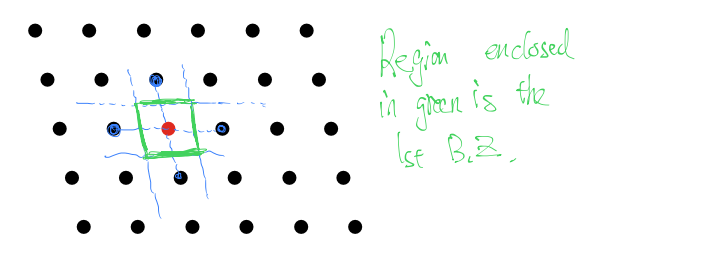
\includegraphics[width=.9\linewidth]{./bz1st.png}
\caption{Area enclosed in green is the first BZ}
\end{figure}


\section{Problem 2}
\label{sec:org85eff07}
From \(S_{\bf{G}} \equiv \sum_{\text{atoms in unit cell}} f_{j}(\bf{G}) e^{i
\bf{G}\cdot \bf{x}_{j}}\), and the question states that: \(\bf{G} = 0 \cdot
\bf{b}_{1} + 0 \cdot \bf{b}_{2} + l \cdot \bf{b}_{3}\). Using \(\bf{b}_{i} \cdot
\bf{a}_{j} = 2\pi \delta_{ij}\) We get

\begin{align}
S_{00l} & = f_{Ba} e^{i * 0} + f_{Ti} e^{i * 1/2 *l * \bf{b}_{3} \cdot \bf{a}_{3} } + f_{O}(e^{i * 0 } + e^{i * 1 / 2 * 0 * \bf{b}_{1} \cdot \bf{a}_{1} + i * 1 / 2 * l * \bf{b}_{3} \cdot \bf{a}_{3}} \\
       &  + e^{i * 1 / 2 * 0 * \bf{b}_{2} \cdot \bf{a}_{2} + i * 1 / 2 * l * \bf{b}_{3} \cdot \bf{a}_{3}}) \\
       & = f_{Ba} + (e^{i\pi})^{l} f_{Ti} + [1 + 2(e^{i\pi})^{l}] f_{O} \\
       & = f_{Ba} + (-1)^{l}f_{Ti} + [1+2(-1)^{l}]f_{O} \qed
\end{align}
\end{document}